\documentclass[conference,a4paper]{IEEEtran}

\IEEEoverridecommandlockouts

\usepackage{cite}
\usepackage{amsmath,amssymb}
\usepackage{graphicx}
\usepackage{booktabs}
\usepackage{array}
\usepackage{multirow}
\usepackage{url}
\usepackage{balance}

\begin{document}

\title{Topology-Prior Guided PCB Transistor Defect Inspection Using ResNet-18 and U-Net Variants}

\author{
\IEEEauthorblockN{Hasan Can Karatepe}
\IEEEauthorblockA{\textit{Dept. of Electrical \& Electronics Engineering} \\
\textit{Abdullah Gul University}\\
Kayseri, Turkiye \\
hasancan.karatepe@agu.edu.tr \\
ORCID: 0009-0009-8221-3141}
}


\maketitle

\begin{abstract}
Automated visual inspection of printed circuit board (PCB) components is important for detecting assembly faults such as bent leads, cut leads, package damage, and component misplacement. Standard computer vision models generally treat all image regions based only on visual appearance, although defects on current-carrying metallic leads are usually more critical than cosmetic variations on the plastic package. This study proposes a two-stage inspection pipeline for transistor defects using the MVTec AD transistor dataset. In the first stage, a ResNet-18 classifier performs image-level Go/No-Go anomaly detection. Synthetic defect images without pixel-level masks are used only for Stage 1 image-level augmentation. In the second stage, pixel-level defect localization is performed using U-Net based segmentation models. Three segmentation variants are compared: an RGB-only U-Net baseline, a Fixed-Prior U-Net using a topology prior as an additional input channel, and a Learnable Topology U-Net. Experimental results show that the synthetic-augmented Stage 1 classifier achieves an AUROC of 0.9911 and an F1-score of 0.8889 on held-out real images. For Stage 2 segmentation, the Fixed-Prior U-Net achieves the best performance, with a defect IoU of 0.6175, mean IoU of 0.8000, and pixel-level AUROC of 0.9771. These results suggest that a simple topology-guided prior can significantly improve defect localization in limited-data PCB inspection settings.
\end{abstract}

\begin{IEEEkeywords}
PCB inspection, anomaly detection, semantic segmentation, U-Net, ResNet-18, topology prior, MVTec AD, computer vision.
\end{IEEEkeywords}

\section{Introduction}

Automated optical inspection is widely used in electronics manufacturing to detect assembly defects before they cause functional failures. For through-hole or power-electronics components, such as transistor packages, small geometric errors may have important electrical consequences. A bent or damaged metallic lead may affect solderability, contact resistance, or electrical continuity, while a visually noticeable mark on the plastic package may be less critical. This creates an important difference between purely visual defect detection and engineering-aware inspection.

Recent industrial anomaly detection methods have achieved strong results on benchmark datasets such as MVTec AD \cite{bergmann2019mvtec,bergmann2021mvtec}. Many of these methods are designed for the normal-sample-only setting and use deep features from pretrained convolutional networks. For example, PatchCore uses a representative memory bank of nominal patch features for anomaly detection and localization \cite{roth2022patchcore}, while PaDiM models patch feature distributions using pretrained CNN embeddings \cite{defard2021padim}. More recent methods, such as ADTR and EfficientAD, investigate transformer-based feature reconstruction or efficient student-teacher anomaly detection \cite{you2022adtr,batzner2024efficientad}. These approaches are effective for generic industrial inspection, but they typically do not explicitly include electrical or topology-based knowledge about which component regions are more important.

In PCB inspection, domain knowledge is often available before training. For example, the approximate location of current-carrying metallic leads can be obtained from package geometry, component datasheets, or PCB footprint information. This motivates the use of a topology prior to guide the segmentation network toward electrically important regions.

This work investigates whether such a simple engineering prior can improve transistor defect localization under limited annotated data. The proposed system has two stages. Stage 1 performs image-level Go/No-Go classification using ResNet-18 \cite{he2016resnet}. Stage 2 performs pixel-level defect segmentation using U-Net based models \cite{ronneberger2015unet}. The study compares an RGB-only U-Net baseline, a Fixed-Prior U-Net, and a Learnable Topology U-Net.

The main contributions of this work are:
\begin{itemize}
    \item A two-stage PCB transistor inspection pipeline is implemented, combining image-level classification and pixel-level semantic segmentation.
    \item A Fixed-Prior U-Net is proposed to incorporate a topology map of electrically critical lead regions into the segmentation model.
    \item A Learnable Topology U-Net is implemented as an ablation to evaluate whether the topology cue can be used through a learnable attention mechanism.
    \item Synthetic defect images are used only for Stage 1 image-level augmentation, while Stage 2 segmentation is trained and evaluated using real images with pixel-level masks.
    \item A quantitative comparison is performed using precision, recall, F1-score, defect IoU, mean IoU, and pixel-level AUROC.
\end{itemize}

The implementation code will be made available in a public GitHub repository \cite{repo2026}.

\section{Materials and Methods}

\subsection{Dataset}

The experiments use the transistor category of the MVTec Anomaly Detection dataset \cite{bergmann2019mvtec,bergmann2021mvtec}. MVTec AD is designed for industrial visual inspection and contains high-resolution images of multiple object and texture categories. The transistor category includes normal samples and defect types such as bent lead, cut lead, damaged case, and misplaced component.

The official MVTec AD setting is mainly unsupervised, where the training set contains normal images and the test set contains both normal and anomalous images. In this project, a supervised re-split was used because the goal was to train and compare segmentation models using available ground-truth defect masks. The real images were split into training, validation, and test sets with a fixed random seed. Healthy images with blank masks were also included in the segmentation training set to teach the U-Net models that normal transistor regions should be considered background.

The 22 synthetic defect images generated during the project did not have pixel-level masks. Therefore, they were used only for Stage 1 image-level classifier augmentation. They were not used for Stage 2 segmentation training, validation, or final testing.

Synthetic defect images were generated by editing real transistor images to create additional image-level faulty examples. The edits were designed to preserve the original camera viewpoint, PCB background, component scale, and lighting while introducing one visible defect pattern such as a bent lead, cut lead, damaged package, or component misplacement. After generation, the images were manually inspected and assigned to defect-type folders. Since these synthetic images did not include pixel-level defect masks, they were used only as faulty image-level samples for Stage 1 classifier augmentation. They were not used for Stage 2 segmentation training, validation, or final testing. This avoids using unverified synthetic masks in the pixel-level evaluation.

\begin{table}[!t]
\centering
\caption{Stage 1 Image-Level Classification Split}
\label{tab:stage1split}
\begin{tabular}{lccc}
\toprule
Class / Defect Type & Train & Validation & Test \\
\midrule
Healthy & 163 & 54 & 56 \\
Bent lead & 5 & 2 & 3 \\
Cut lead & 5 & 2 & 3 \\
Damaged case & 5 & 2 & 3 \\
Misplaced & 5 & 2 & 3 \\
\midrule
Total real images & 183 & 62 & 68 \\
Synthetic faulty images & 22 & 0 & 0 \\
\bottomrule
\end{tabular}
\end{table}

\begin{table}[!t]
\centering
\caption{Stage 2 Pixel-Level Segmentation Split}
\label{tab:stage2split}
\begin{tabular}{lccc}
\toprule
Class / Defect Type & Train & Validation & Test \\
\midrule
Healthy empty-mask images & 40 & 16 & 24 \\
Bent lead & 5 & 2 & 3 \\
Cut lead & 5 & 2 & 3 \\
Damaged case & 5 & 2 & 3 \\
Misplaced & 5 & 2 & 3 \\
\midrule
Total images & 60 & 24 & 36 \\
\bottomrule
\end{tabular}
\end{table}

\begin{figure}[!t]
    \centering
    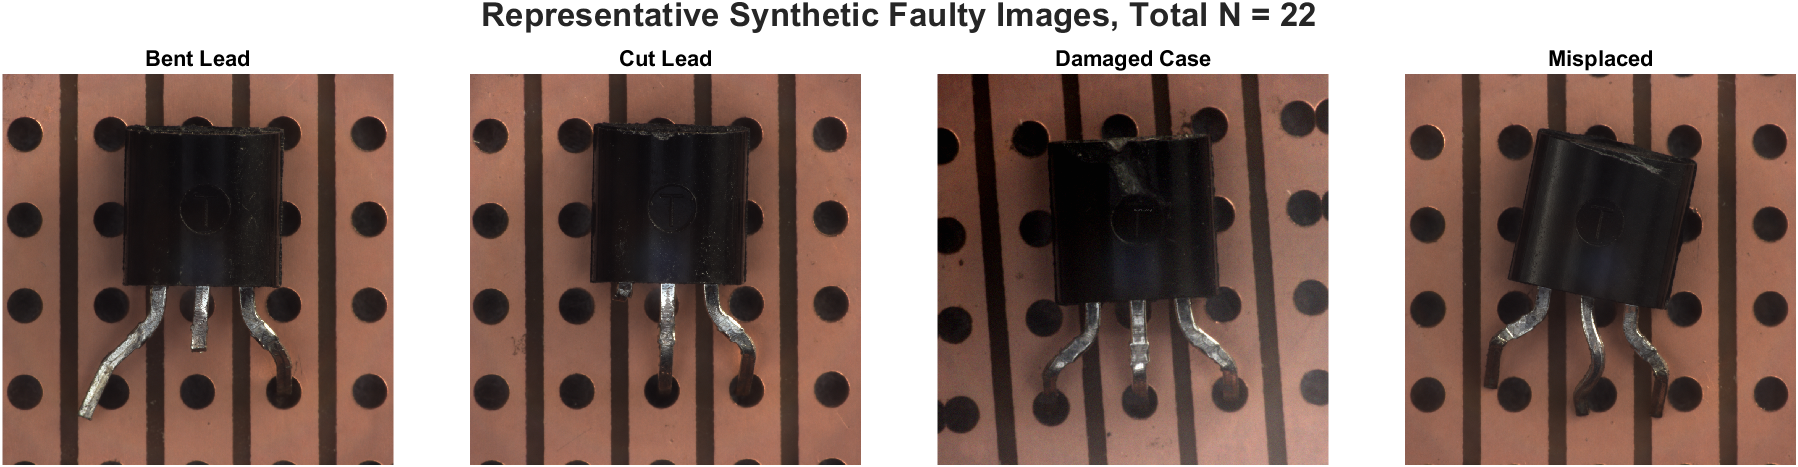
\includegraphics[width=\linewidth]{fig_synthetic_examples.png}
    \caption{Representative synthetic faulty transistor images used only for Stage 1 image-level classifier augmentation. These images were not used for Stage 2 segmentation because pixel-level masks were unavailable.}
    \label{fig:synthetic}
\end{figure}

\subsection{Overall Pipeline}

Fig.~\ref{fig:pipeline} shows the proposed two-stage inspection pipeline. The first stage acts as a fast Go/No-Go classifier. If the component is classified as potentially faulty, the second stage performs semantic segmentation to localize defective pixels.

\begin{figure*}[!t]
    \centering
    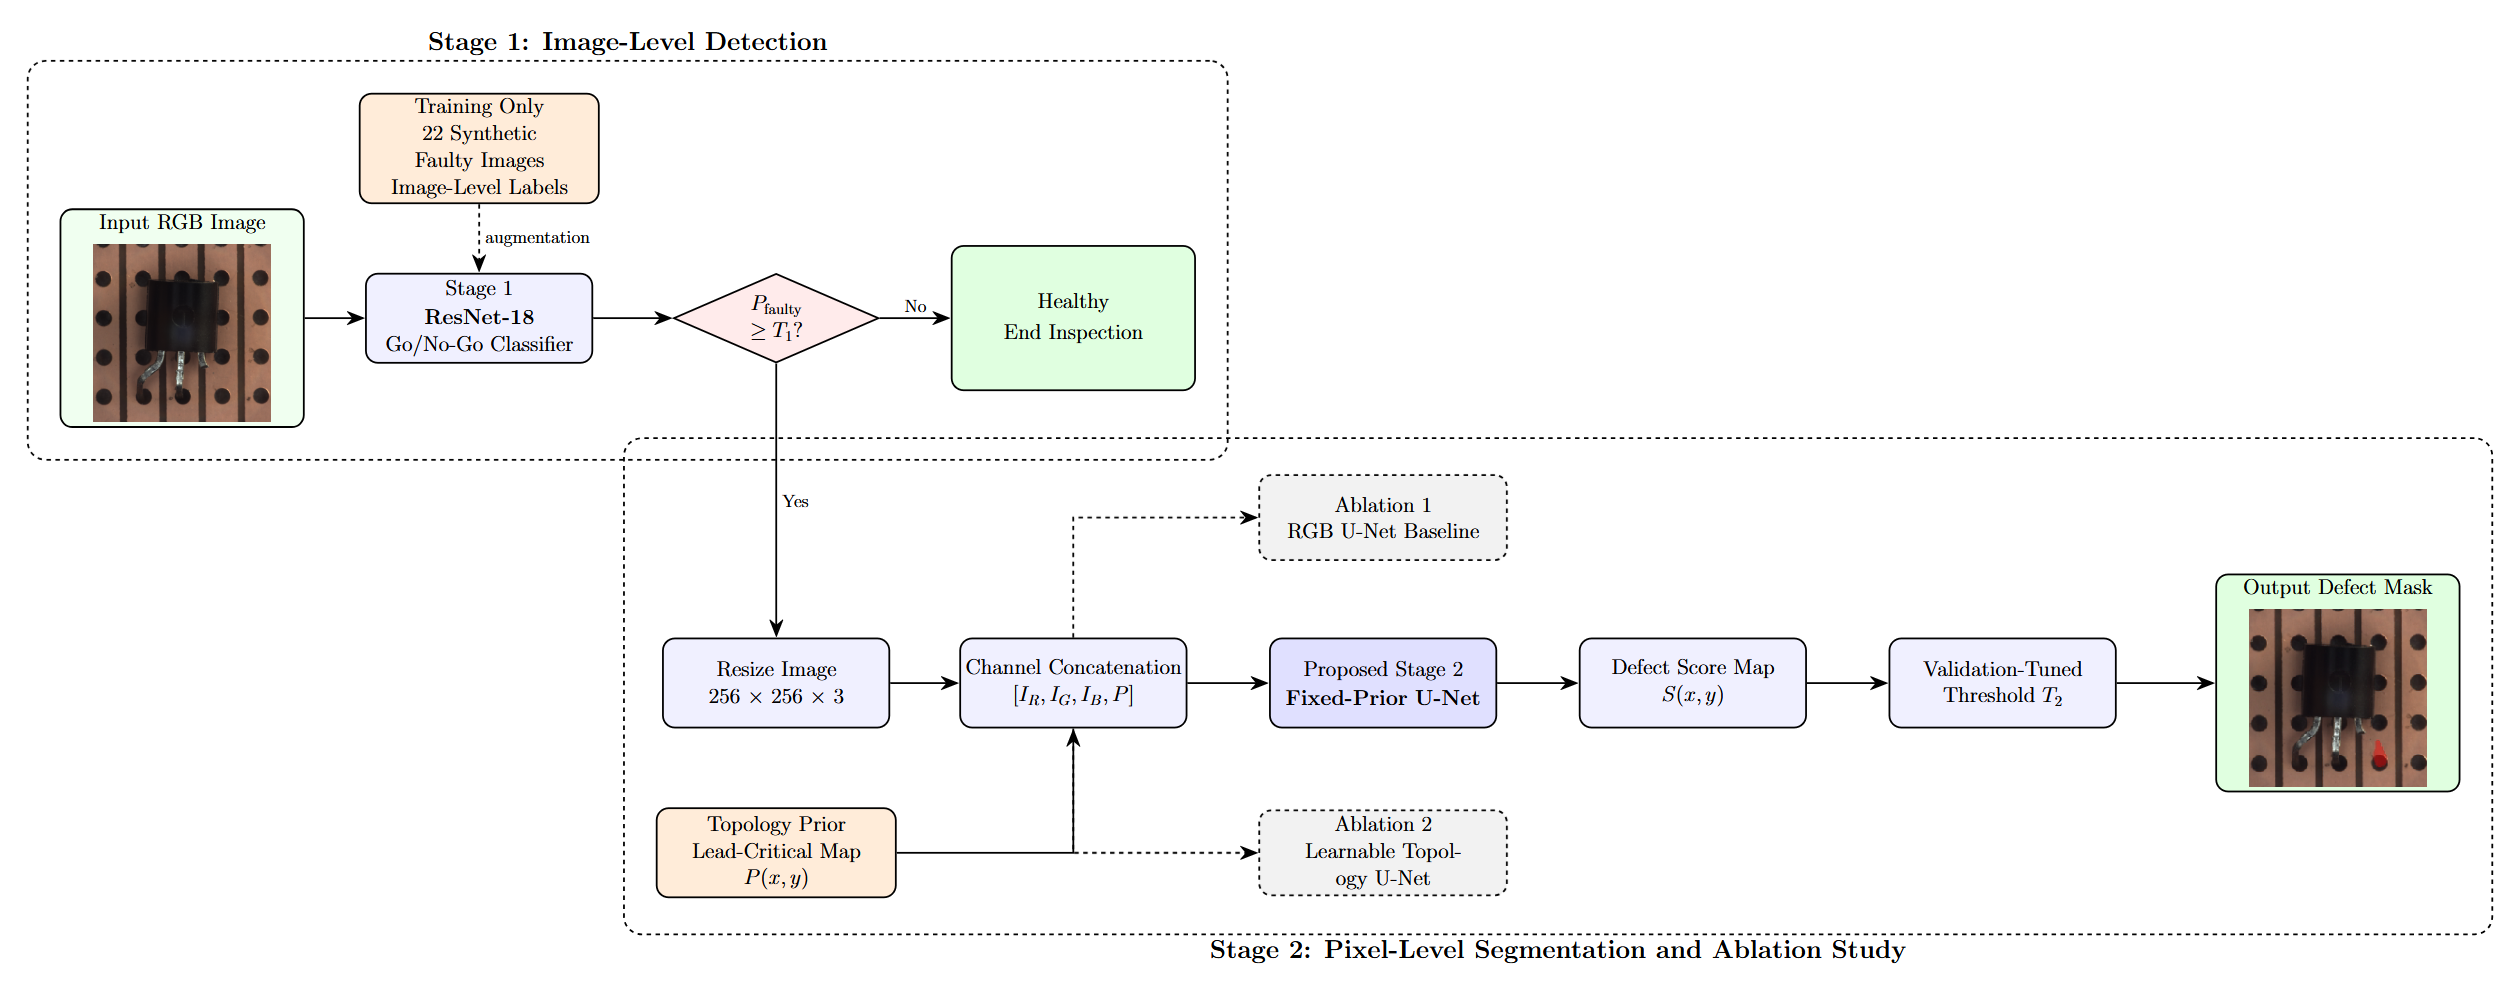
\includegraphics[width=\textwidth]{fig_pipeline.png}
    \caption{Proposed two-stage inspection pipeline. Stage 1 performs image-level Go/No-Go classification using ResNet-18. If the component is classified as potentially faulty, Stage 2 performs pixel-level segmentation. The main proposed segmentation model is the Fixed-Prior U-Net, while the RGB U-Net and Learnable Topology U-Net are evaluated as ablation models.}
    \label{fig:pipeline}
\end{figure*}

\subsection{Stage 1: Image-Level Go/No-Go Classification}

Stage 1 uses ResNet-18 as a binary classifier. The output classes are Healthy and Faulty. Input images are resized to $224 \times 224$ pixels. The network is trained using the Adam optimizer with an initial learning rate of $10^{-4}$, mini-batch size of 16, and 10 epochs.

Because the inspection objective prioritizes not missing defective components, the default classifier decision threshold was not used directly. Instead, the faulty-class probability threshold was selected on the validation set by maximizing F1-score. The selected threshold was then applied to the held-out test set.

\subsection{Stage 2: Semantic Segmentation Models}

Stage 2 performs pixel-level defect segmentation. Three U-Net based variants are evaluated.

\subsubsection{RGB U-Net Baseline}

The RGB U-Net baseline receives only the resized RGB image as input:
\begin{equation}
X_{\mathrm{RGB}} \in \mathbb{R}^{256 \times 256 \times 3}.
\end{equation}
This model serves as the purely data-driven segmentation baseline.

\subsubsection{Fixed-Prior U-Net}

The Fixed-Prior U-Net receives the RGB image concatenated with a topology prior channel:
\begin{equation}
X_{\mathrm{fixed}} = [I_R, I_G, I_B, P],
\end{equation}
where $P \in [0,1]^{256 \times 256}$ is the topology prior. High values in $P$ correspond to expected current-carrying metallic lead regions, while lower values correspond to the plastic package and background. Fig.~\ref{fig:prior} shows the topology prior used in this study.

\begin{figure}[!t]
    \centering
    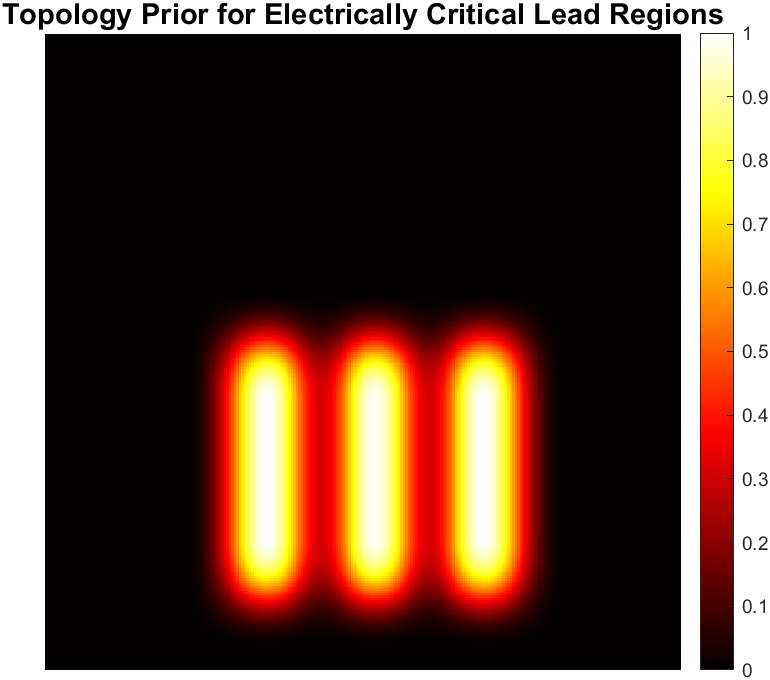
\includegraphics[width=0.85\linewidth]{fig_topology_prior.png}
    \caption{Topology prior used by the Fixed-Prior U-Net. The high-priority regions correspond to expected current-carrying transistor leads.}
    \label{fig:prior}
\end{figure}

The prior was generated from the approximate transistor geometry in the MVTec images. Rectangular lead regions were assigned high weights and then smoothed using a Gaussian filter. This prior is not intended to be a final decision mask; instead, it gives the network an additional topology cue.

\subsubsection{Learnable Topology U-Net}

To address the scalability limitation of a fixed handcrafted prior, a learnable topology-conditioned variant was also implemented. This model receives the same four-channel input, but the prior is used through a learnable attention layer before the U-Net. The RGB image is modulated as
\begin{equation}
I' = I \odot \left(1 + \sigma(\alpha)P\right),
\end{equation}
where $I$ is the RGB image, $P$ is the topology prior, $\alpha$ is a learnable scalar parameter, $\sigma(\cdot)$ is the sigmoid function, and $\odot$ denotes element-wise multiplication. This formulation allows the network to learn how strongly the topology prior should influence the image features.

\subsection{Training Parameters}

All models were implemented in MATLAB using the Deep Learning Toolbox and trained on a workstation GPU equipped with an NVIDIA Quadro P2000. The Stage 1 ResNet-18 classifier used an input size of $224 \times 224$ pixels, Adam optimizer, initial learning rate of $10^{-4}$, mini-batch size of 16, and 10 training epochs.

The Stage 2 U-Net models used an input size of $256 \times 256$ pixels and encoder depth of 4. The Adam optimizer was used with an initial learning rate of $10^{-4}$, mini-batch size of 8, and 80 epochs. To reduce the effect of class imbalance, weighted pixel classification loss was used. The RGB and Fixed-Prior U-Nets used class weights of 1.0 for background and 3.0 for defect. The Learnable Topology U-Net used a smaller defect weight of 2.0 because it was more prone to over-segmentation.

For each segmentation model, the defect probability threshold was selected on the validation set by maximizing F1-score. The selected threshold was then applied to the held-out test images. Table~\ref{tab:trainingtime} summarizes the approximate training time of each model on the Quadro P2000 GPU.

\begin{table}[!t]
\centering
\caption{Approximate Training Time on NVIDIA Quadro P2000 GPU}
\label{tab:trainingtime}
\begin{tabular}{lc}
\toprule
Training Step & Approx. Training Time \\
\midrule
Stage 1 ResNet-18 classifier & 1 min 45 s \\
RGB U-Net baseline & 13 min 30 s \\
Fixed-Prior U-Net & 14 min 14 s \\
Learnable Topology U-Net & 13 min 45 s \\
\midrule
Total training time & 43 min 14 s \\
\bottomrule
\end{tabular}
\end{table}

\subsection{Evaluation Metrics}

Stage 1 classification was evaluated using accuracy, precision, recall, F1-score, and AUROC. For Stage 2 segmentation, the following metrics were used: precision, recall, F1-score, defect intersection-over-union (IoU), mean IoU, and pixel-level AUROC.

The defect IoU is defined as
\begin{equation}
\mathrm{IoU}_{defect} = \frac{TP}{TP + FP + FN},
\end{equation}
where $TP$, $FP$, and $FN$ are computed at the pixel level. Mean IoU is computed as the average IoU of the background and defect classes.

\subsection{Custom PCB Image Collection Protocol}

Although the experimental results in this paper are based on MVTec AD, a custom PCB image collection protocol was also defined for future extension. Images should be collected using a fixed camera-to-board distance, fixed illumination, and a top-down view. Normal samples should contain correctly placed components, while defective samples should include controlled cases such as bent leads, cut or thinned leads, damaged packages, and component misplacement. Pixel-level masks should be created using a manual labeling tool. The data should be split at the board level into training, validation, and test sets to avoid leakage between visually similar samples. For new component types, the topology prior can be generated from datasheets, CAD footprints, or reference images.

\section{Experimental Results}

\subsection{Stage 1 Classification Results}

Table~\ref{tab:stage1} presents the Stage 1 results. Synthetic defect images were used only as image-level faulty samples during classifier training. The final evaluation was performed on real held-out images.

\begin{table}[!t]
\centering
\caption{Stage 1 Synthetic-Augmented ResNet-18 Classification Results}
\label{tab:stage1}
\begin{tabular}{lc}
\toprule
Metric & Value \\
\midrule
Selected threshold & 0.07 \\
Accuracy & 0.9559 \\
Precision & 0.8000 \\
Recall & 1.0000 \\
F1-score & 0.8889 \\
AUROC & 0.9911 \\
TP / FP / FN / TN & 12 / 3 / 0 / 53 \\
\bottomrule
\end{tabular}
\end{table}

The classifier achieved perfect recall on the test set, meaning that no defective sample was missed. This behavior is desirable in an inspection pipeline, because a false negative may allow a defective component to pass into later manufacturing stages. The cost is a small number of false positives, which are less critical because flagged samples can be passed to Stage 2 or human inspection.

Fig.~\ref{fig:stage1roc} shows the ROC curve, and Fig.~\ref{fig:stage1cm} shows the threshold-tuned confusion matrix.

\begin{figure}[!t]
    \centering
    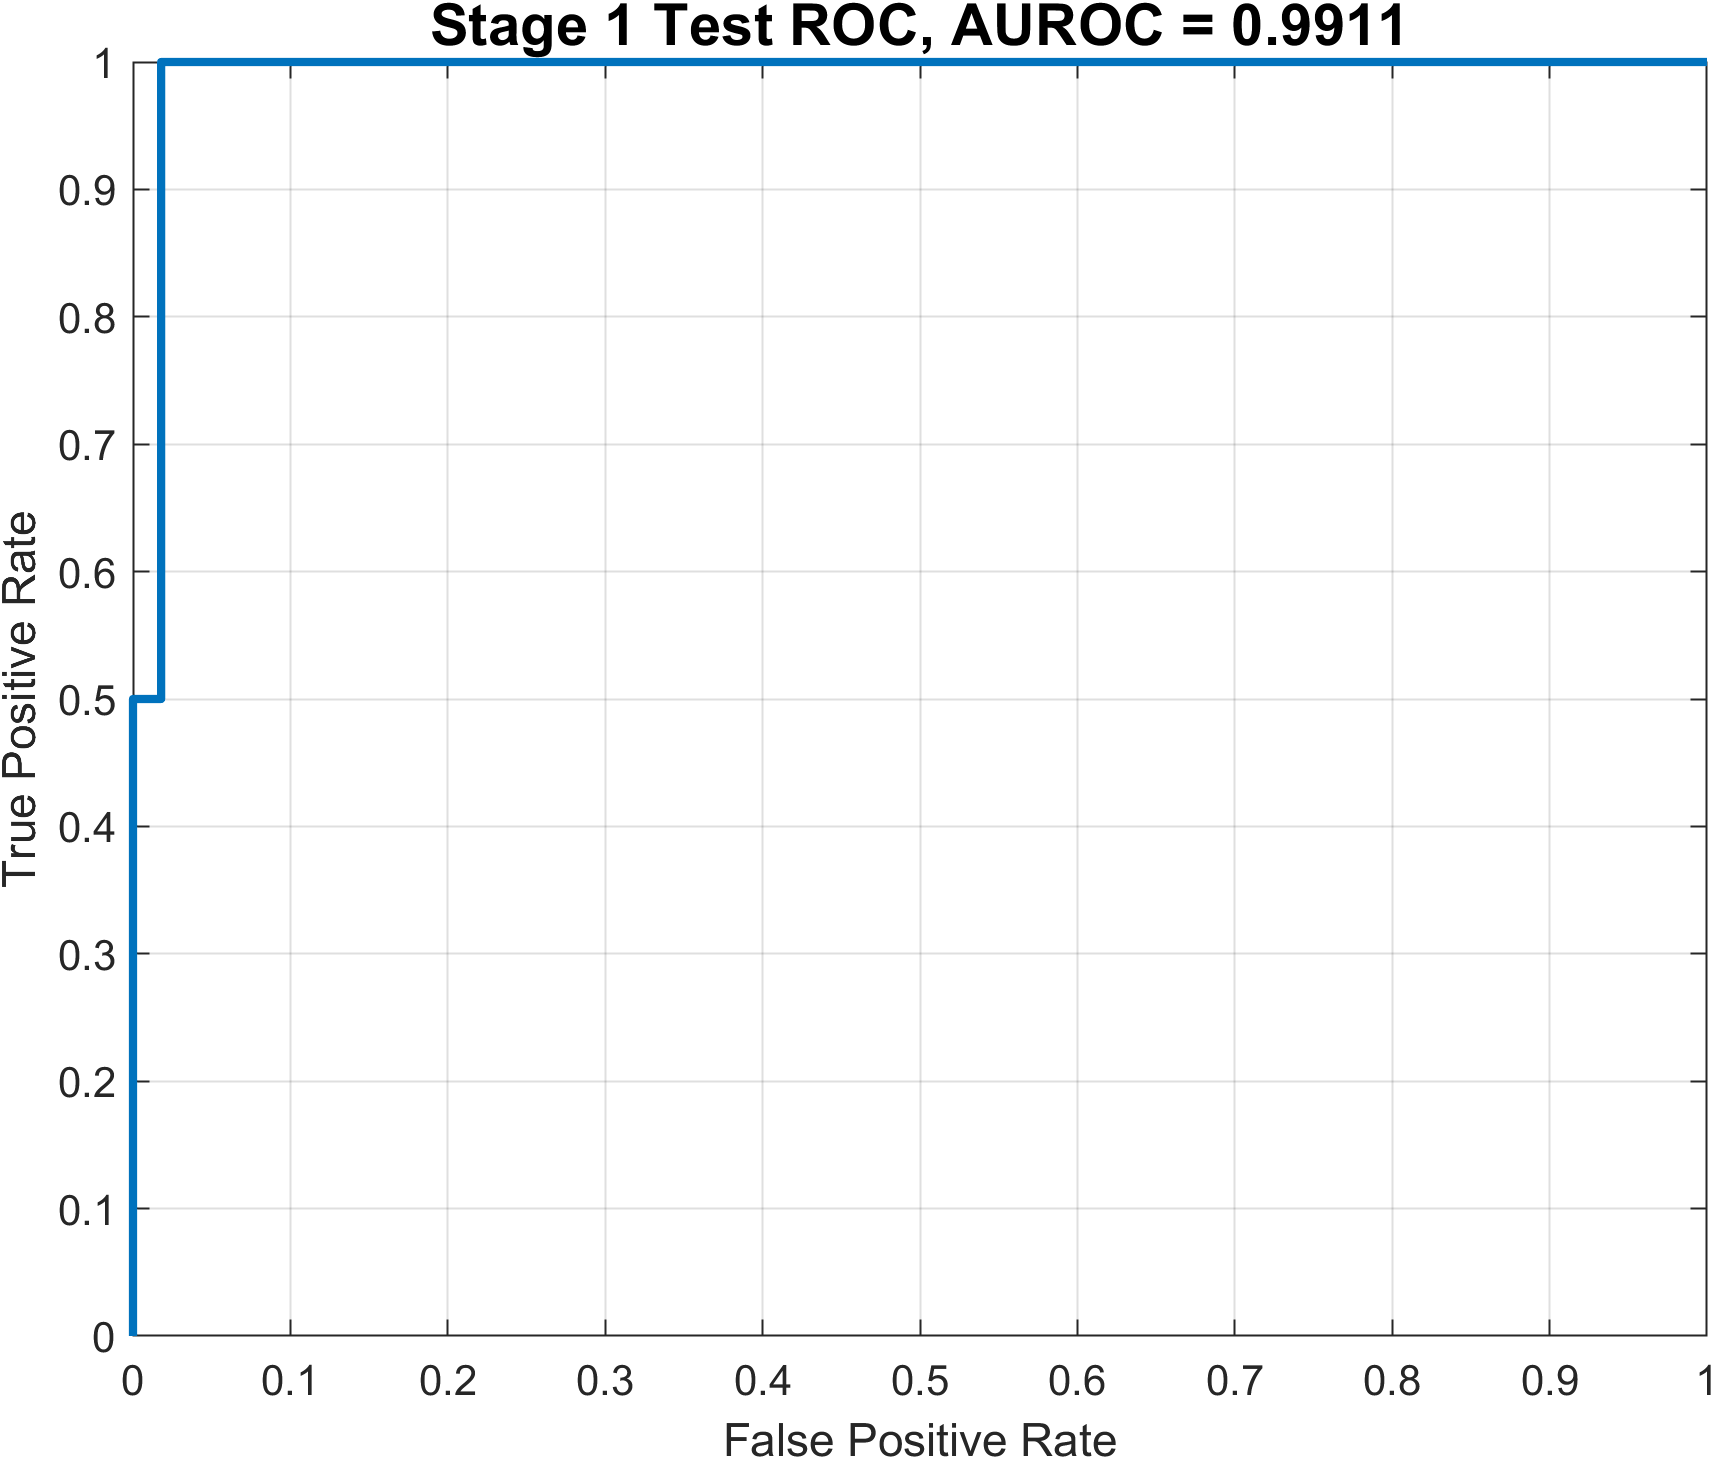
\includegraphics[width=\linewidth]{fig_stage1_roc.png}
    \caption{ROC curve of the Stage 1 synthetic-augmented ResNet-18 classifier.}
    \label{fig:stage1roc}
\end{figure}

\begin{figure}[!t]
    \centering
    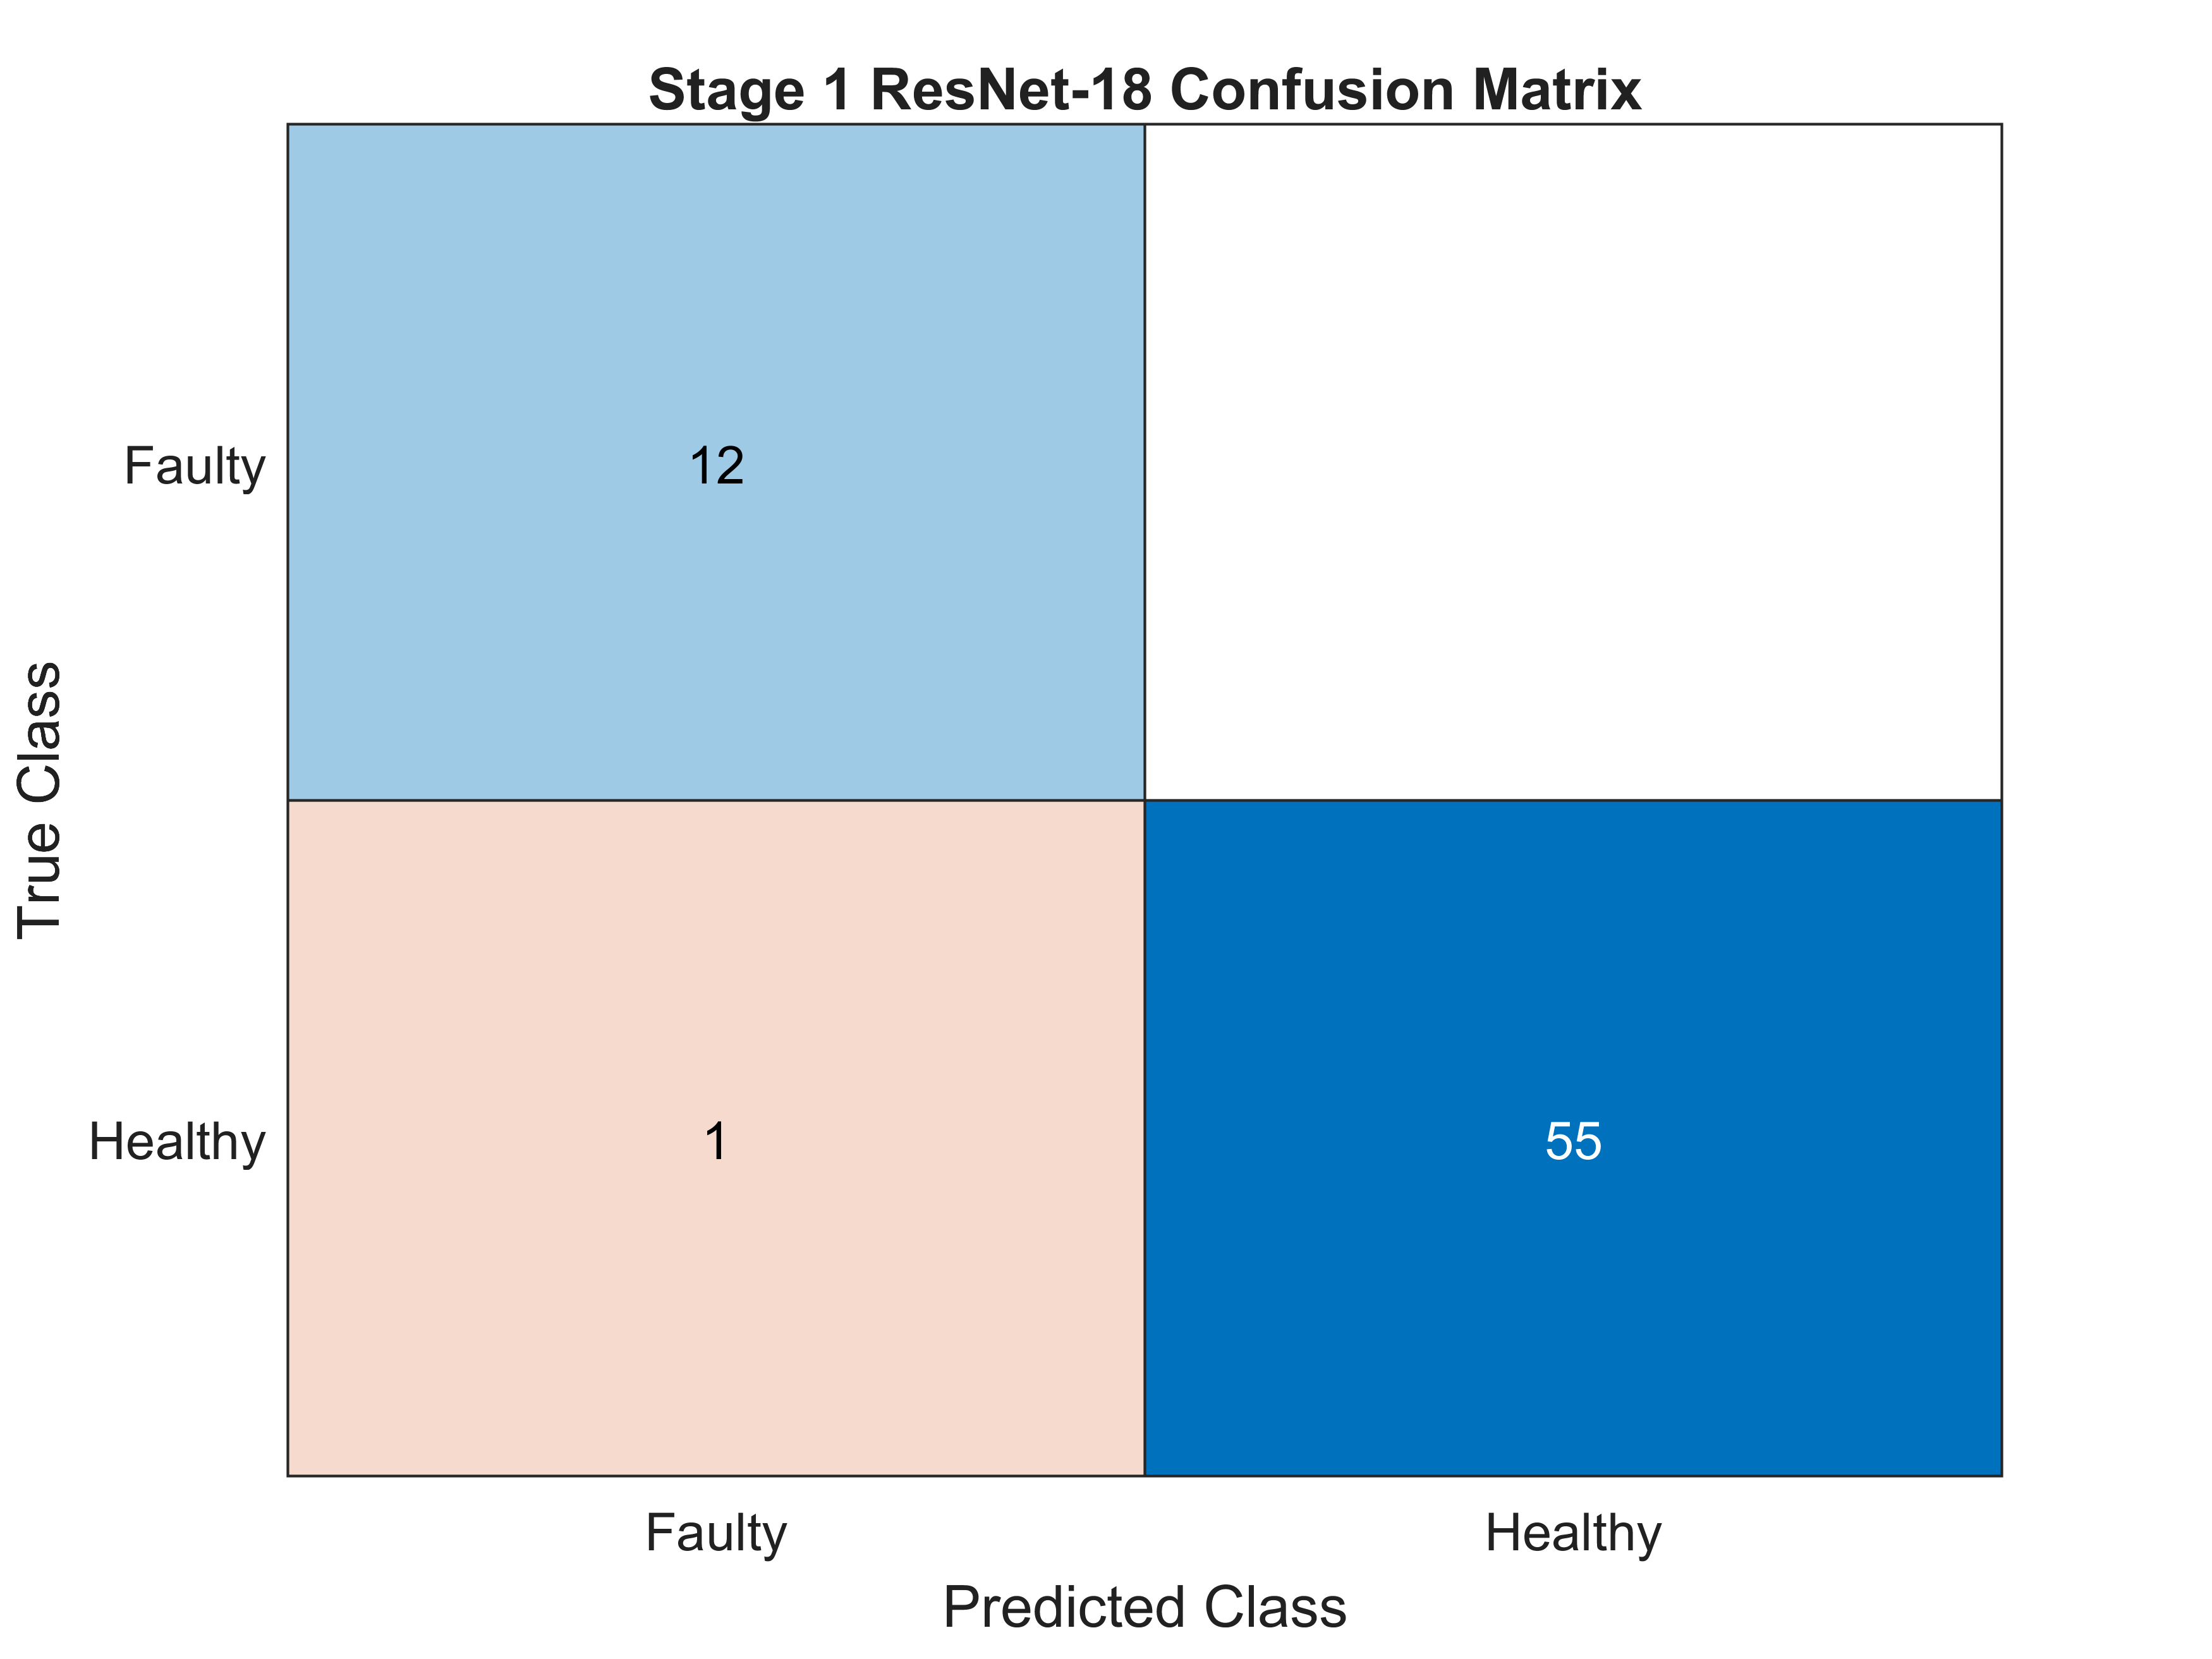
\includegraphics[width=0.85\linewidth]{fig_stage1_confusion.png}
    \caption{Threshold-tuned Stage 1 confusion matrix. The selected threshold prioritizes defect recall.}
    \label{fig:stage1cm}
\end{figure}

\subsection{Stage 2 Segmentation Results}

Table~\ref{tab:stage2} shows the final segmentation results. These experiments were conducted using real MVTec images with pixel-level masks. The synthetic images were not used for segmentation because they did not have defect masks.

\begin{table*}[!t]
\centering
\caption{Stage 2 Segmentation Results on Real Held-Out MVTec Images}
\label{tab:stage2}
\begin{tabular}{lccccccc}
\toprule
Model & Threshold & Precision & Recall & F1-score & Defect IoU & Mean IoU & Pixel AUROC \\
\midrule
RGB U-Net Baseline & 0.34 & 0.3435 & 0.4862 & 0.4026 & 0.2520 & 0.5975 & 0.8869 \\
Fixed-Prior U-Net & 0.95 & \textbf{0.8298} & \textbf{0.7071} & \textbf{0.7635} & \textbf{0.6175} & \textbf{0.8000} & \textbf{0.9771} \\
Learnable Topology U-Net & 0.17 & 0.4714 & 0.5721 & 0.5169 & 0.3485 & 0.6531 & 0.8120 \\
\bottomrule
\end{tabular}
\end{table*}

The Fixed-Prior U-Net achieved the best performance in all reported Stage 2 metrics. Compared with the RGB-only U-Net baseline, defect IoU improved from 0.2520 to 0.6175. The F1-score also improved from 0.4026 to 0.7635. This indicates that the topology prior helped the network reject false positives and localize defects more accurately.

The Learnable Topology U-Net also improved over the RGB-only baseline in defect IoU and F1-score, but it did not outperform the Fixed-Prior U-Net. This suggests that the learnable topology mechanism was useful, but less stable under the limited number of annotated defect masks. In this small-data setting, the explicit fixed prior provided stronger guidance than the learnable attention mechanism.

Fig.~\ref{fig:ablation} summarizes the ablation results.

\begin{figure}[!t]
    \centering
    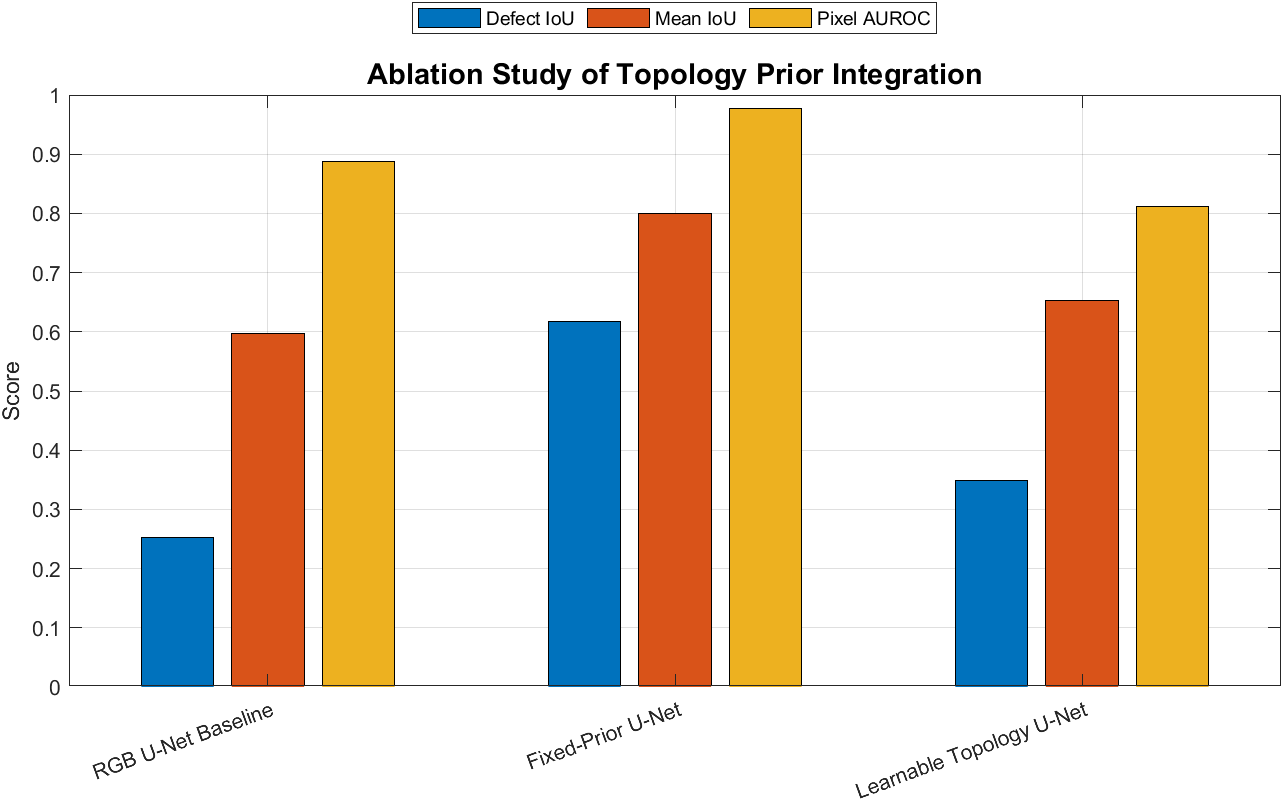
\includegraphics[width=\linewidth]{fig_stage2_ablation.png}
    \caption{Ablation comparison of RGB U-Net, Fixed-Prior U-Net, and Learnable Topology U-Net.}
    \label{fig:ablation}
\end{figure}

\begin{table}[!t]
\centering
\caption{Relative Improvement of Fixed-Prior U-Net over RGB U-Net}
\label{tab:improvement}
\begin{tabular}{lc}
\toprule
Metric & Relative Improvement \\
\midrule
F1-score & 89.6\% \\
Defect IoU & 145.0\% \\
Mean IoU & 33.9\% \\
Pixel AUROC & 10.2\% \\
\bottomrule
\end{tabular}
\end{table}

Table~\ref{tab:improvement} summarizes the relative improvement of the Fixed-Prior U-Net over the RGB-only U-Net baseline. The largest gain is observed in defect IoU, which confirms that the topology prior mainly improves spatial localization accuracy.

\subsection{Qualitative Results}

Fig.~\ref{fig:qualitative} shows representative qualitative results for different defect types. The RGB U-Net baseline often activates on visually strong but non-defective regions. The Fixed-Prior U-Net generally produces more localized masks and better agreement with the ground-truth defect regions. This supports the quantitative results in Table~\ref{tab:stage2}.

\begin{figure*}[!t]
    \centering
    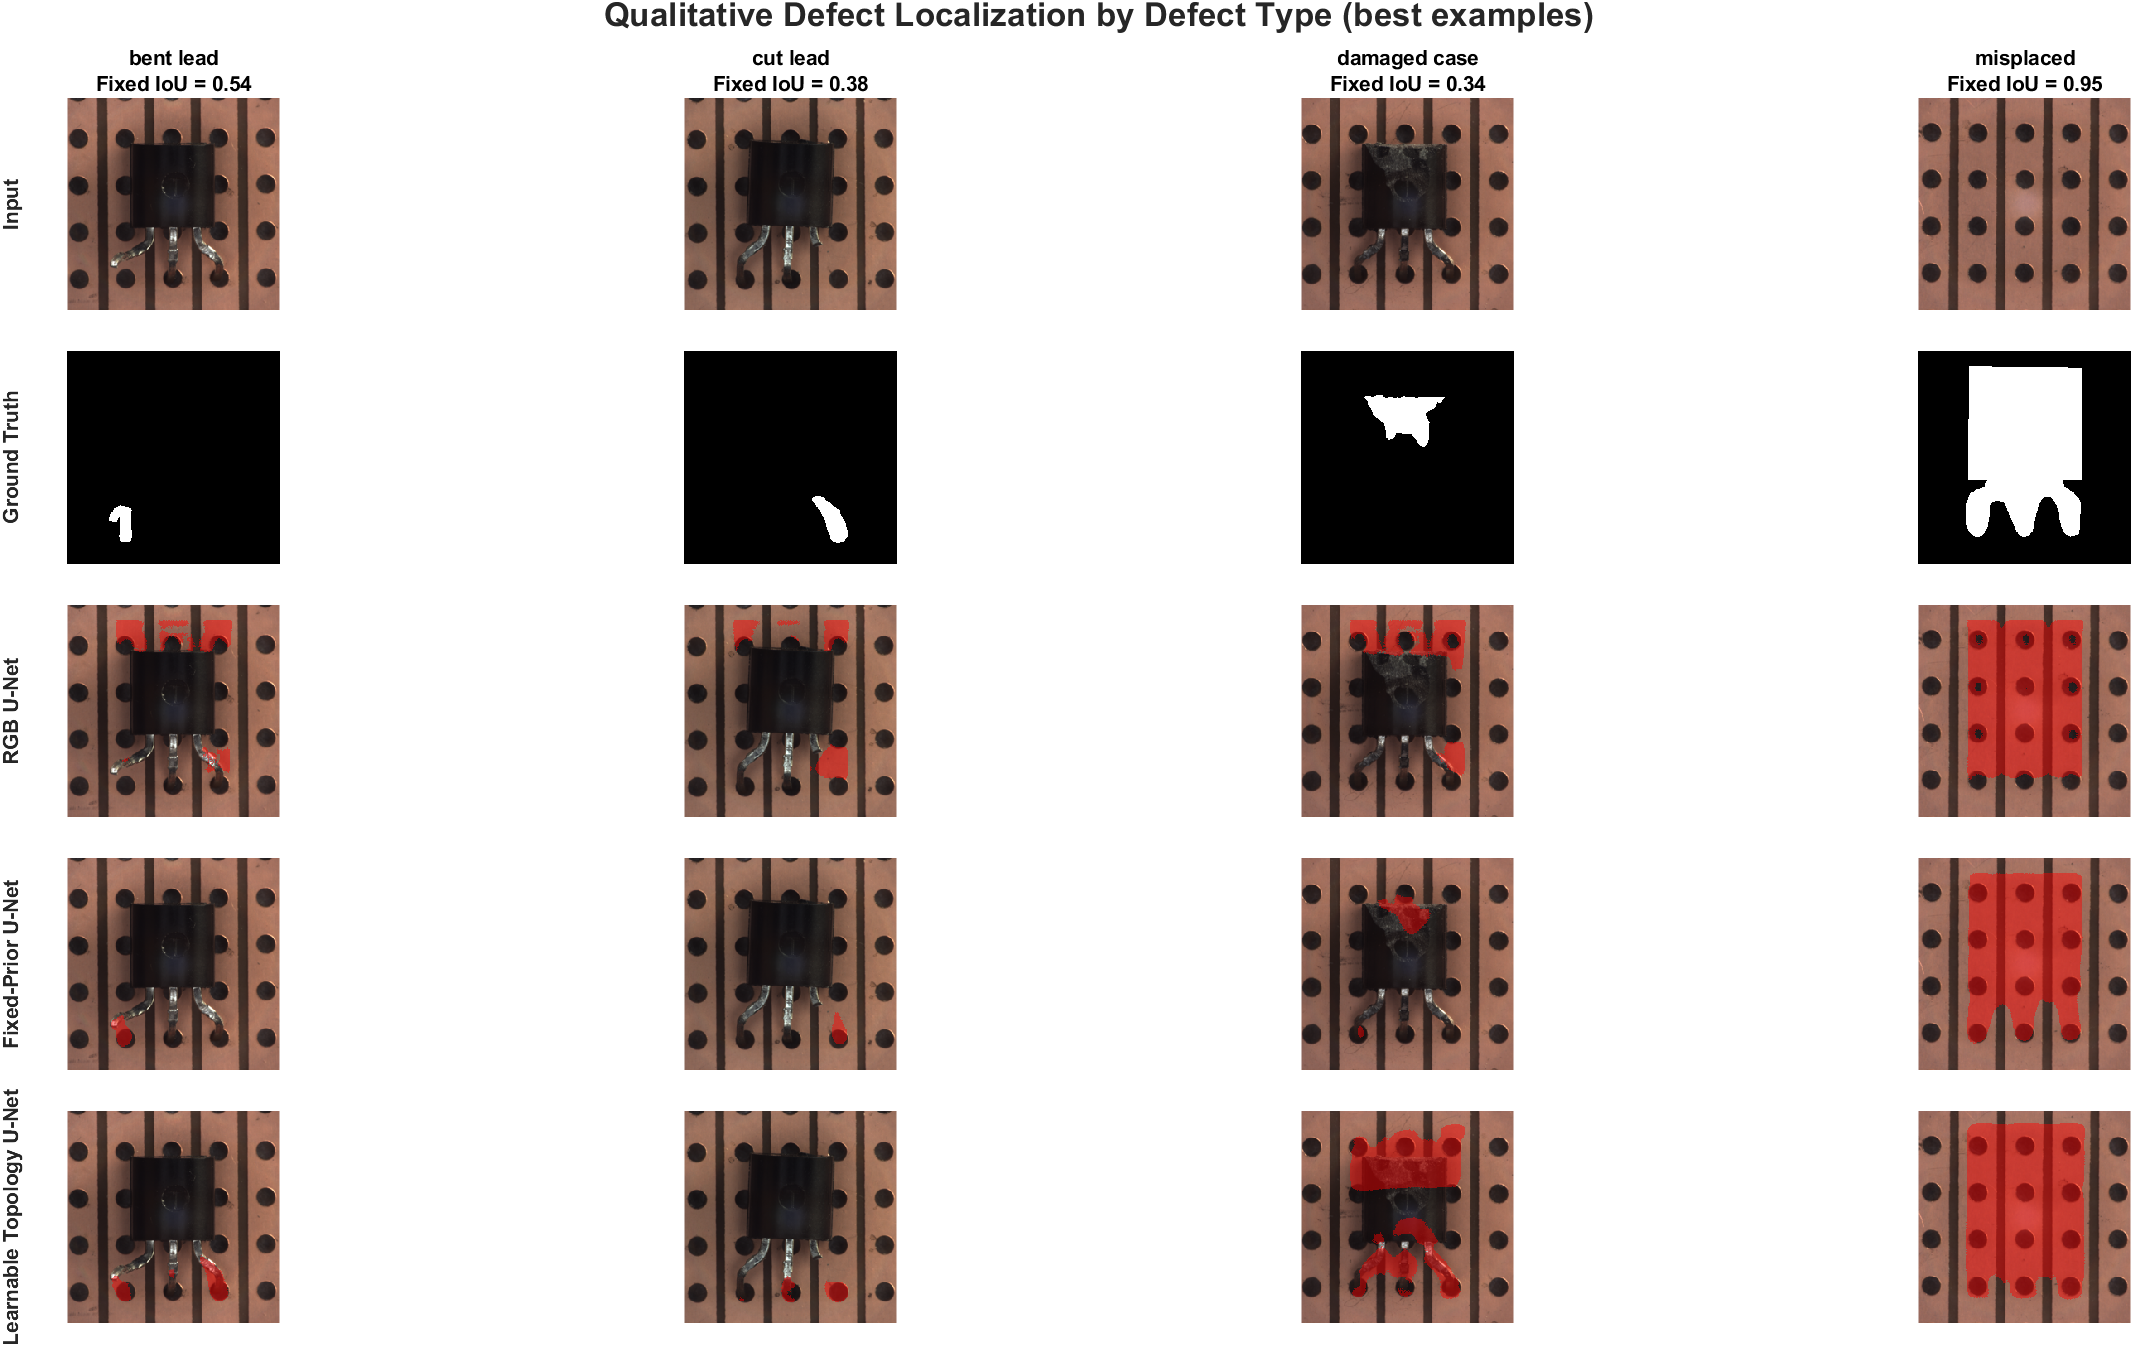
\includegraphics[width=\textwidth]{fig_qualitative.png}
    \caption{Qualitative segmentation examples by defect type. The Fixed-Prior U-Net provides the most accurate localization among the tested models.}
    \label{fig:qualitative}
\end{figure*}

Fig.~\ref{fig:heatmaps} shows defect score heatmaps for representative defect types. These heatmaps provide additional insight beyond the final binary masks. The Fixed-Prior U-Net generally produces stronger and more localized responses near the annotated defect regions, while the RGB-only and learnable topology variants show more diffuse activations. This supports the numerical improvement observed in defect IoU and pixel-level AUROC.

\begin{figure*}[!t]
    \centering
    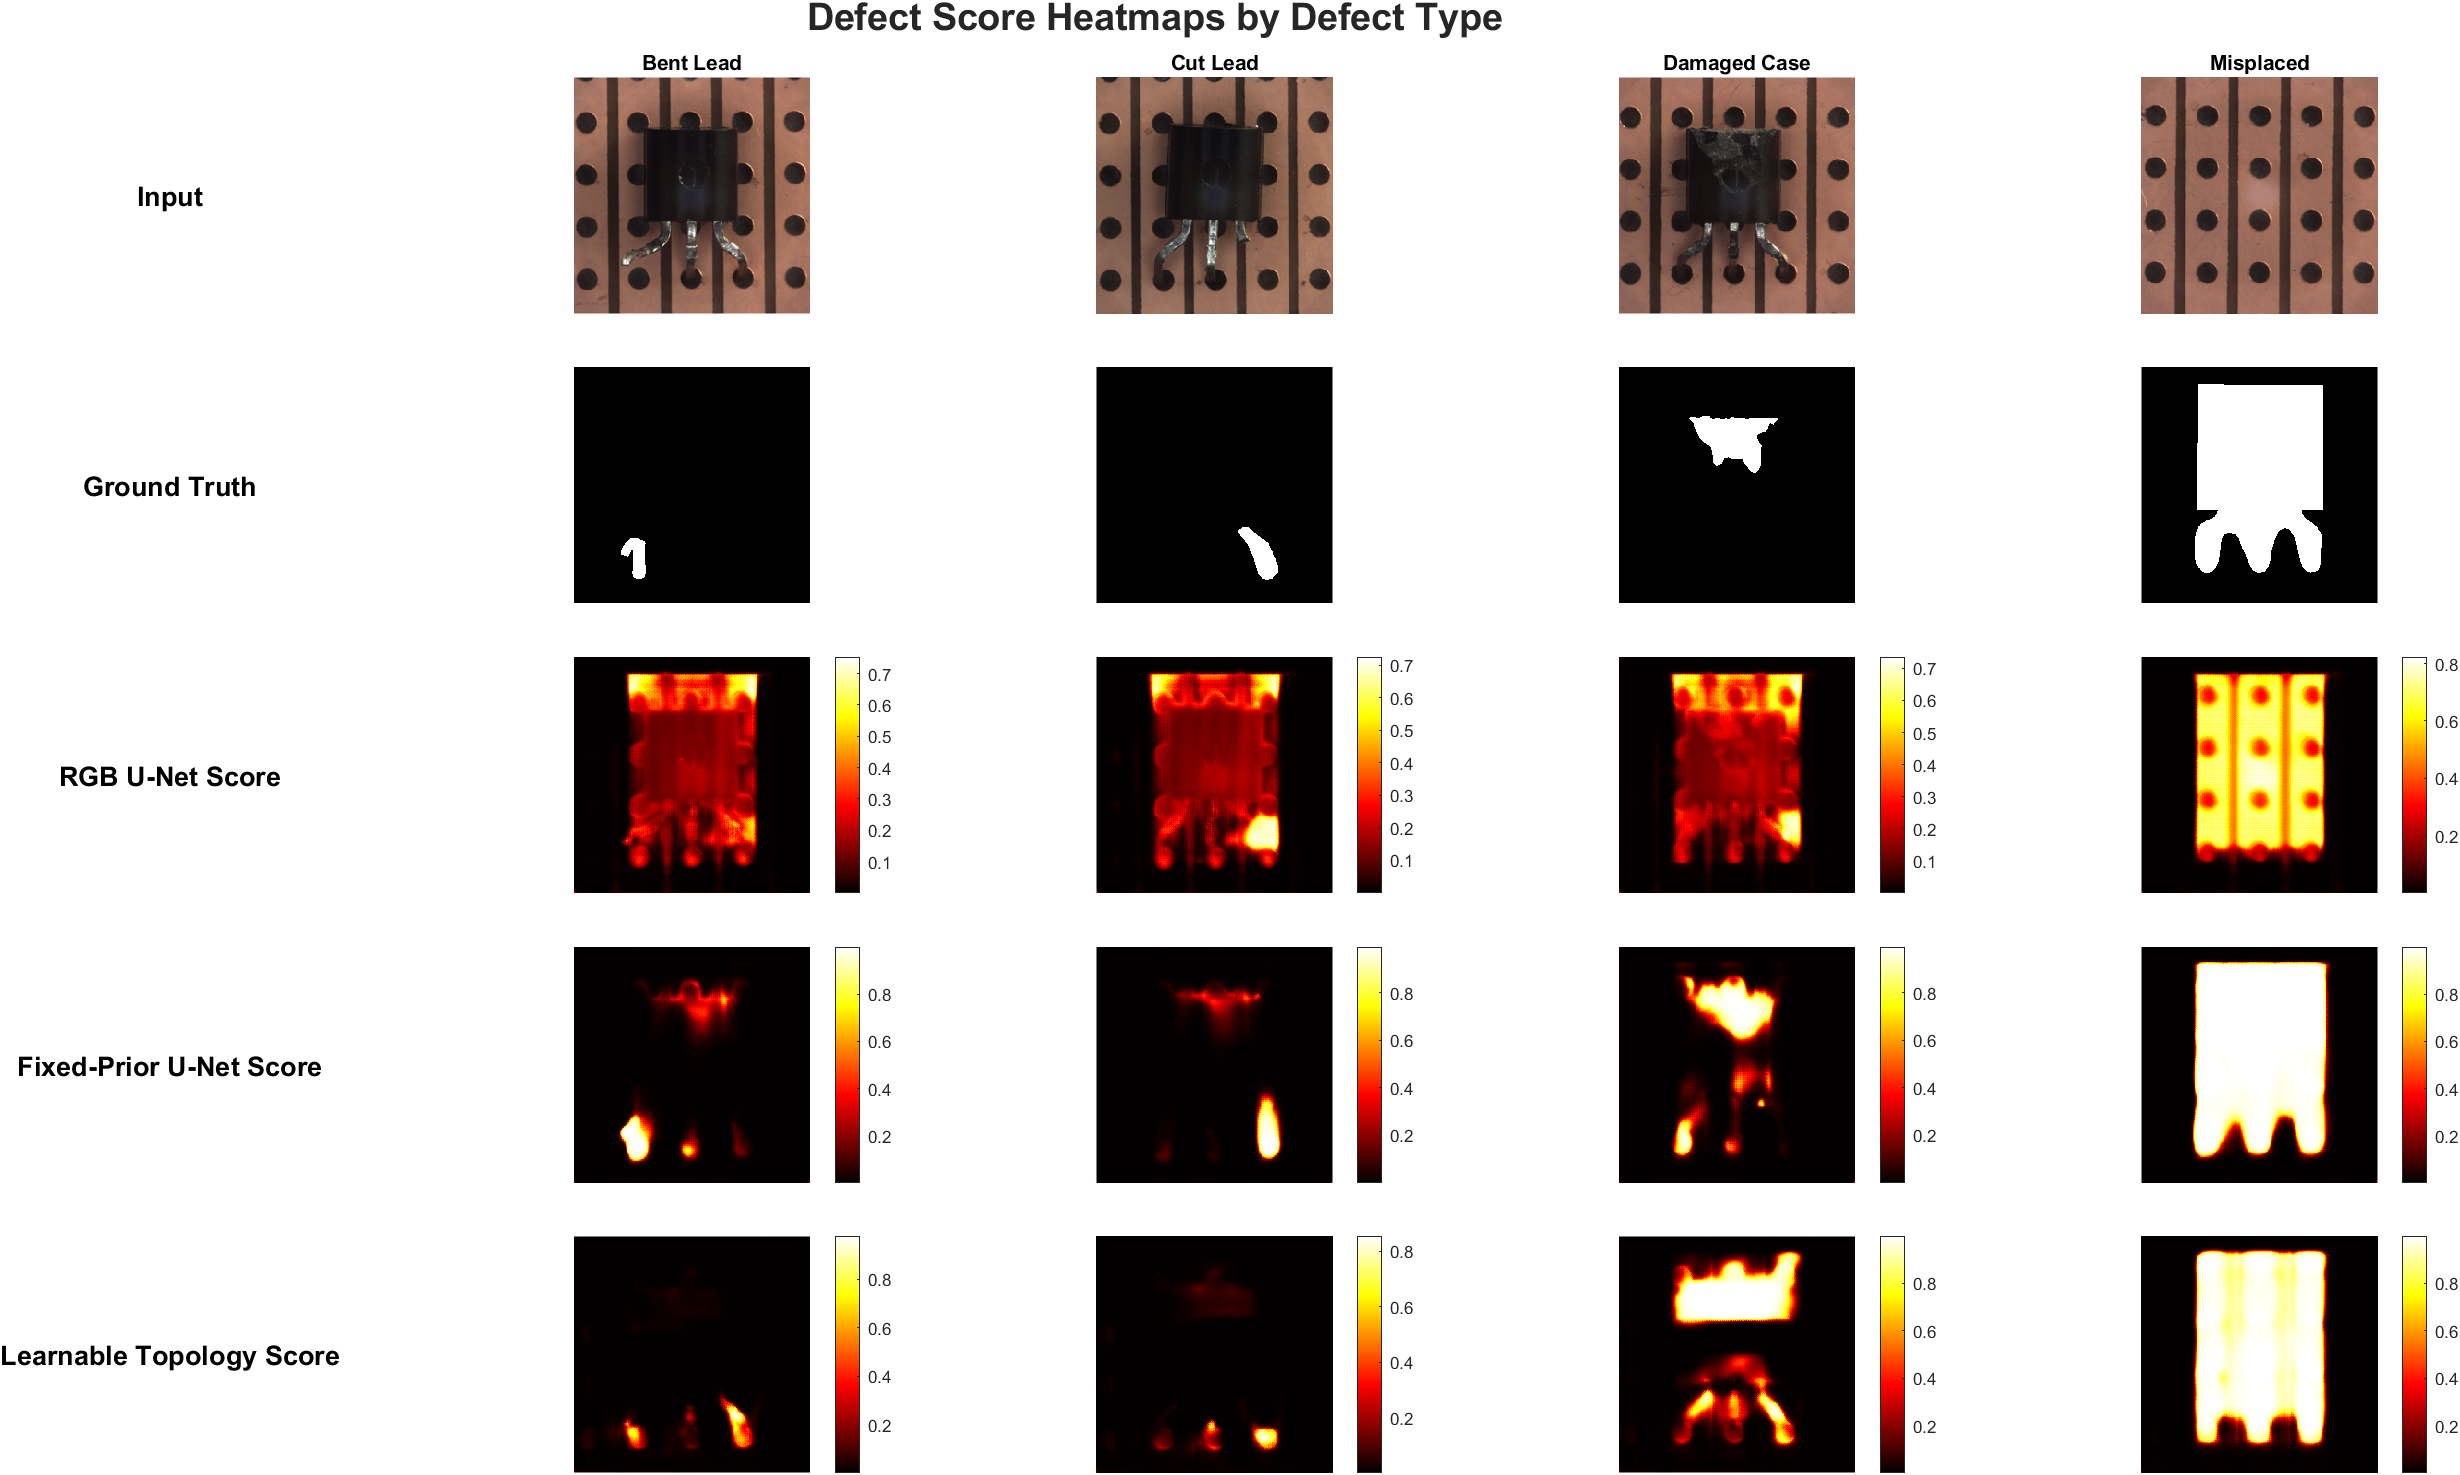
\includegraphics[width=\textwidth]{fig_heatmaps.png}
    \caption{Defect score heatmaps for different defect types. The Fixed-Prior U-Net produces more concentrated responses around defect regions compared with the other variants.}
    \label{fig:heatmaps}
\end{figure*}

\subsection{Effect of Threshold Tuning}

Threshold tuning had a noticeable effect on both stages. For Stage 1, the threshold was selected to improve defect recall, which is important in inspection tasks. For Stage 2, each model used a validation-selected defect probability threshold. The Fixed-Prior U-Net selected a high threshold of 0.95, indicating that its defect probability map was confident and allowed aggressive false-positive suppression. This contributed to its high precision and strong IoU score.

\begin{figure}[!t]
    \centering
    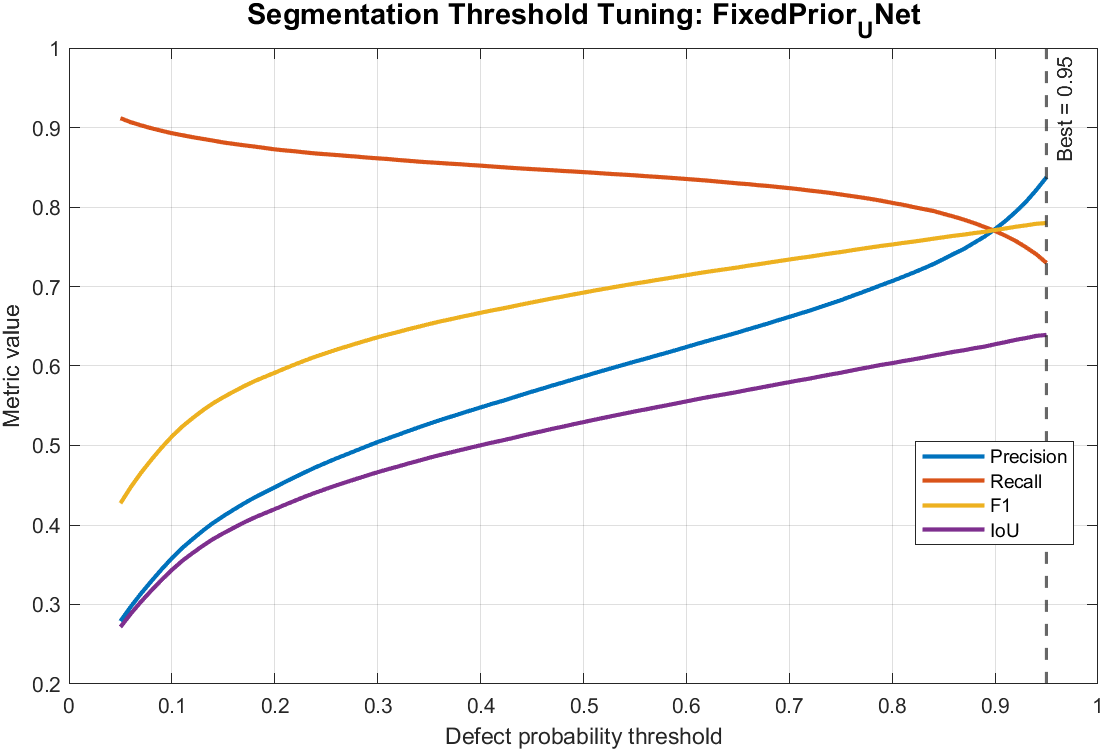
\includegraphics[width=\linewidth]{fig_threshold_fixed.png}
    \caption{Validation-based threshold tuning for the Fixed-Prior U-Net. The selected threshold improves the precision-recall tradeoff for defect localization.}
    \label{fig:thresholdfixed}
\end{figure}

As shown in Fig.~\ref{fig:thresholdfixed}, threshold tuning is important because the default semantic segmentation output may over-segment visually strong but non-defective regions. For the Fixed-Prior U-Net, the selected high threshold helped suppress false positives while preserving the most confident defect regions.

\section{Discussion}

The results support the main hypothesis of this study: incorporating simple topology information can improve defect localization in PCB transistor inspection. The Fixed-Prior U-Net substantially outperformed the RGB-only baseline. This is reasonable from an electrical engineering perspective, because lead regions are both visually relevant and functionally important. The additional topology channel gave the model a useful spatial cue that was not available to the RGB-only baseline.

The Learnable Topology U-Net was included to address the limitation of a fixed handcrafted prior. Although it improved over the RGB baseline, it underperformed the Fixed-Prior U-Net. One possible reason is that the dataset is too small for the attention branch to learn a robust spatial weighting strategy. In contrast, the fixed prior gives direct guidance and does not require additional parameters to learn the location of critical regions.

There are several limitations. First, the study uses only the transistor category of MVTec AD. Therefore, the generalization of the topology prior to other component types was not experimentally verified. Second, the fixed prior is based on approximate component alignment and may not work well if the component is shifted, rotated, or imaged under a different setup. Third, synthetic images were used only for Stage 1 because pixel-level masks were unavailable. If synthetic images are manually labeled in future work, they could also be used to improve Stage 2 segmentation. Finally, the topology prior mainly emphasizes lead-critical defects. Some package-level defects, such as damaged casing, may require a different or multi-region prior.

The additional topology-prior input did not introduce a large computational burden. The Fixed-Prior U-Net required approximately 14 min 14 s to train, compared with 13 min 30 s for the RGB-only U-Net baseline on the same NVIDIA Quadro P2000 GPU.

A small robustness check was conducted to evaluate the sensitivity of the Fixed-Prior U-Net to image-prior misalignment. In this experiment, the Stage 2 test images and ground-truth masks were artificially shifted by $\pm 10$ pixels or rotated by $\pm 5^\circ$, while the topology prior was kept fixed. This intentionally simulates a mismatch between the assumed lead locations and the actual component position. As shown in Table~\ref{tab:robustness}, the original aligned case achieved the highest defect IoU of 0.6175. Performance decreased under all perturbations, especially for the +10 pixel shift, where defect IoU dropped to 0.2677. Interestingly, recall remained relatively high in several perturbed cases, but precision decreased, indicating that the model produced more false-positive pixels when the image and prior were misaligned. This confirms that the fixed prior is useful under controlled alignment, but future work should estimate component pose or generate the topology prior dynamically from detected component geometry.

\begin{table}[!t]
\centering
\caption{Robustness of Fixed-Prior U-Net}
\label{tab:robustness}
\begin{tabular}{lccc}
\toprule
Condition & F1 & Defect IoU & Mean IoU \\
\midrule
Original & 0.7635 & 0.6175 & 0.8000 \\
Shift +10 px & 0.4223 & 0.2677 & 0.5944 \\
Shift -10 px & 0.5886 & 0.4170 & 0.6881 \\
Rotate +5$^\circ$ & 0.6165 & 0.4456 & 0.7060 \\
Rotate -5$^\circ$ & 0.6837 & 0.5194 & 0.7459 \\
\bottomrule
\end{tabular}
\end{table}

The robustness experiment confirms that the method is sensitive to image-prior misalignment, so a practical deployment should include component registration, pose correction, or dynamic prior generation.

Future work should evaluate the approach on custom PCB images collected under controlled imaging conditions. The topology map can also be generated automatically from CAD footprints or datasheets instead of manually defining approximate regions. A more advanced learnable attention model could integrate the topology prior at multiple encoder levels rather than only at the input. This would better address scalability to different component types and package geometries.

\section{Conclusion}

This paper presented a topology-prior guided two-stage inspection pipeline for transistor defects in PCB images. The first stage used a synthetic-augmented ResNet-18 classifier for image-level Go/No-Go detection and achieved an AUROC of 0.9911 and an F1-score of 0.8889. The second stage compared three U-Net based segmentation models on real MVTec images with ground-truth masks. The Fixed-Prior U-Net achieved the best segmentation performance, with a defect IoU of 0.6175, mean IoU of 0.8000, and pixel-level AUROC of 0.9771. These results show that even a simple topology prior can provide useful engineering guidance for defect localization in limited-data inspection problems.

\section*{Acknowledgment}

The initial project proposal structure and wording were developed with assistance from Google Gemini. OpenAI ChatGPT was used for MATLAB code review, debugging assistance, report organization, and language refinement. Mistral Le Chat was used during the proposal stage for feasibility checking. The author reviewed and verified the generated content, experimental results, and references, and takes full responsibility for the final submission.

\balance
\bibliographystyle{IEEEtran}
\bibliography{references}

\end{document}